% !TEX root = MAIN.tex

\chapter{\DAMA - Validation Execution Environment Definition and Results}

\begin{figure}[h]
  \centering
  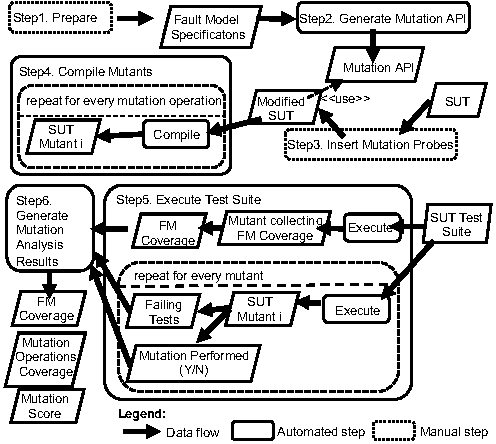
\includegraphics[width=0.6\textwidth]{images/dataDrivenBufferProcess.pdf}
      \caption{DAMAt methodology.}
      \label{fig:damat}
\end{figure}

Figure~\ref{fig:damat} introduces \DAMA methodology.
Validation was performed by applying the \DAMA methodology to the case studies listed in the \emph{SPAP} document (chapter 5):
\begin{itemize}
  \item LXS System Test Suite for ESAIL.
  \item GSL System Test Suite for LibParam.
\end{itemize}

Particularly, we verified that \DAMA complied with the requirements expressed in the \emph{Software System Specification} (\emph{SSS}), section 4.1.1.
The validation procedures and tasks are described in the \emph{Software Validation Specification} (\emph{SVS}) document, Section 5.2.


\begin{table}[h]
\caption{MASS Validation Report.}
\label{table:damat:results}
\scriptsize
\centering
\begin{tabular}{|@{\hspace{1pt}}p{33mm}|
@{\hspace{1pt}}>{\raggedleft\arraybackslash}p{12mm}@{\hspace{1pt}}|
>{\raggedleft\arraybackslash}p{12mm}@{\hspace{1pt}}|
>{\raggedleft\arraybackslash}p{12mm}@{\hspace{1pt}}|
}
\hline
\textbf{Task}&\textbf{ESAIL}&\textbf{libparam}\\
\hline
Instrumenting the source code - \DAMA&PASSED&PASSED\\
Configuring and running \emph{\DAMA\_compile.sh} &PASSED&PASSED\\
Configuring and running \emph{\DAMA\_run\_test.sh}&PASSED&PASSED\\
Configuring and running \emph{\DAMA\_obtain\_coverage.sh}&PASSED&PASSED\\
Configuring and running \emph{\DAMA\_mutants\_launcher.sh}&PASSED&PASSED\\
\hline
\end{tabular}

\end{table}



% Particularly, we verified that \DAMA was able to:
% \begin{enumerate}
% 	\item Parse a fault model prepared by the user.
% 	\item Generate a mutation API with the functions that modify the data according to the provided fault model.
%   \item Modify the buffer through calls to the mutation API.
% 	\item Generate and compile mutants.
% 	\item Execute the test suite against all the mutants and gather the results of the test cases.
% 	\item Generate the results of the mutation analysis.
% \end{enumerate}

% \begin{table}[h]
% \caption{MASS Validation Report.}
% \label{table:damat:results}
% \scriptsize
% \centering
% \begin{tabular}{|@{\hspace{1pt}}p{33mm}|
% @{\hspace{1pt}}>{\raggedleft\arraybackslash}p{12mm}@{\hspace{1pt}}|
% >{\raggedleft\arraybackslash}p{12mm}@{\hspace{1pt}}|
% >{\raggedleft\arraybackslash}p{12mm}@{\hspace{1pt}}|
% >{\raggedleft\arraybackslash}p{12mm}@{\hspace{1pt}}|
% }
% \hline
% \textbf{Methodology Step}&\textbf{ESAIL}&\textbf{libgscsp}&\textbf{libparam}\\
% \hline
% Parse the fault model&PASSED&PASSED&PASSED\\
% Generate the mutation &PASSED&PASSED&PASSED\\
% Modify the buffer&PASSED&PASSED&PASSED\\
% Generate and compile the mutants&PASSED&PASSED&PASSED\\
% Execute the test suite&PASSED&PASSED&PASSED\\
% Generate the results&PASSED&PASSED&PASSED\\
% \hline
% \end{tabular}
%
% \end{table}
%
% The idea was to verify that every step of the methodology produced the correct input/outputs. For this reason, we provide Table~\ref{table:damat:results}, that shows the success/failure of every \DAMA step on the different case studies.
%
% A detailed exposition of the validation results is presented in the \emph{D4} document (Chapter 2).

\clearpage
